\documentclass[tikz,border=4pt]{standalone}
\usetikzlibrary{matrix,arrows.meta}
\begin{document}
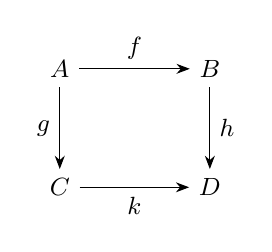
\begin{tikzpicture}[>=Stealth, every node/.style={font=\small}]
  \matrix (m) [matrix of math nodes, row sep=3em, column sep=4em] {
    A & B \\
    C & D \\
  };
  \draw[->] (m-1-1) -- node[above] {$f$} (m-1-2);
  \draw[->] (m-1-1) -- node[left] {$g$} (m-2-1);
  \draw[->] (m-1-2) -- node[right] {$h$} (m-2-2);
  \draw[->] (m-2-1) -- node[below] {$k$} (m-2-2);
\end{tikzpicture}
\end{document}
